%% Los cap'itulos inician con \chapter{T'itulo}, estos aparecen numerados y
%% se incluyen en el 'indice general.
%%
%% Recuerda que aqu'i ya puedes escribir acentos como: 'a, 'e, 'i, etc.
%% La letra n con tilde es: 'n.

\chapter{Results}
\newpage

The following section is dedicated to expose the results obtained after using the developed \textit{Measure System}. The validation of the system is determined by the obtained results. In case the results are valid, the system could be applied to future studies.\\

There is a comparison of the results obtained with the ideal model used by this study. The ideal model is the base to determine if the developed system is applicable to future studies.\\

This section explains the selected use case to test the system. With the obtained information it is possible to decide if it is affordable to use the developed system in future studies.

\section{Studied cases}

The purpose of this project is to find a solution that can be used to study the properties of soils. The solution has to obtain accurate measures, manageable and affordable to apply it to new use cases.\\

This section describes a real use case used to test the system. The chosen use case allow us to determine if the solution obtains realistic values or not. This use case has an amount of values based on time which allow to analyze if the results are valid or not.\\

The variations of the measures produced by the sensors are important too. These variations are critical to decide if the used sensors are appropriated for the system.\\

There are lot of factors which can modified the results acquired:

\begin{itemize}

\item Inclination of the physic scale model. The humidity will change depending on how tilted is the substratum. Depending on the area we are analyzing, the measures could change.

\item Current state of the sensors. The sensors could be damaged if they are connected for a long time. It is not the same to use a new sensor to use a degraded sensor which was connected to the system since months.

\item Soil type used in the study. Depending on the soil types included in the study, the results could change getting different values. Each soil type has a different drying behaviour along time. It is relevant for the study because the produced values could change.

\item Environmental temperature. If there are changes in the environmental temperatures the results can vary. If the environmental temperature is constant the results will follow the ideal model used for the study.

\end{itemize}

To do this study, it was designed a physic scale model of an earth embankment with different soils. This prototype has filters made by other soils like gravel or soils with other granularity properties. The prototype simulates an inclined terrain where the drying process changes depending on the concentration of the water when the terrain wets.

\section{Analysis of the obtained results}

After studying the exposed use cases presented in the system, the obtained results are studied to decide if the system can be used for future studies where materials are involved.\\

To do this study, a representation of the information is requited. This representation has to be done with graphs that can allow us to determine if the measures are reliable or not.\\

The results obtained have to be compared with results obtained by accurate systems. The results obtained by other systems have to be represented in graphs too. To do this comparison, our graphs are built with the information monitored by the system. These graphs are done with Microsoft Excel. To build these graphs, a selection of the monitored information is required. This selection includes information where the changes associated to the humidity of the soil are presented. The evolution of the humidity of the soil depends on the time where the measure was done.\\

When the selection is done, it is required to select the desired graph to represent the selected information. The chosen graph allows to compare the results with other studies or measures.\\

%METER AQUI GRÁFICAS DEL SISTEMA NUESTRO
The figure \ref{Ideal dried graphic} \cite{secado_ideal} represents the ideal dried graphic used as reference. This graph represents how the values can change on an ideal study.\\

\begin{figure}[H]
\begin{centering}
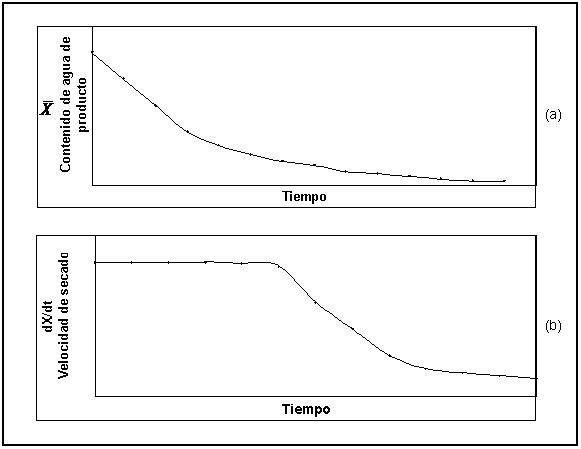
\includegraphics[scale=0.6]{IMGS/secado_ideal.jpg}
\caption{Ideal dried graphic \label{Ideal dried graphic}}
\end{centering}
\end{figure}

As it is possible to see, this picture allows us to know how is the evolution of the measure when the time changes.\\

Having an overview of the ideal studies, the developed system is compared to the ideal model. The goal of this study is to demonstrate if the developed system fulfills to the theorerical models. The measures obtained by the system are represented in the figure \ref{Soil Moisture Evolution in an Earth Dam}.

\begin{figure}[H]
\begin{centering}
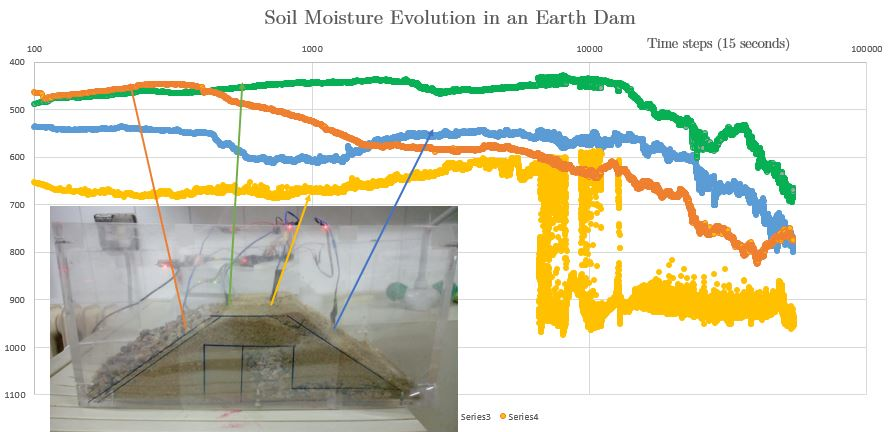
\includegraphics[scale=0.6]{IMGS/results_measures.jpeg}
\caption{Soil Moisture Evolution in an Earth Dam \label{Soil Moisture Evolution in an Earth Dam}}
\end{centering}
\end{figure} 

This graph represents the evolution of the humidity of the soil during the time. There are four humidity sensors connected to the chosen soil. These sensors are allocated in different positions to obtain values depending on the inclination. The prototype represents a real use case, where the inclination is considered and affects to the measured values.\\

Depending on the inclination, the humidity changes. Higher values are tied to the driest values of the soil, and lower values represent the higher humidity values. The evolution of the humidity of the soil depends on time. Also, the chosen prototype has an amount of soils. These soils are the following:\\

\begin{itemize}

\item Soil with gravel.
\item Soil with big granularity.
\item Soil with filter.
\item Normal soil.

\end{itemize}

The behaviour of the drying process depends on the type of the used soil. Soils with filters dry faster than soils without filters. Also, the granularity of the soil influences on the drying process. Soils with more granularity dry faster than soils with few granularity.\\

The prototype has four humidity sensors, which are represented with four colours. The values associated to the used sensors are described as follows:

\begin{itemize}

\item Orange sensor. This sensor dries faster than the other sensors although it is located next to the water. The soil measured by this sensor has a bigger granularity which allows a faster drying process. The granularity of a soils determines how fast it dries.

\item Green sensor. The core of the prototype is measured by this sensor. This core maintains the humidity better than the other measured parts although it wets slowlier than the other soils.

\item Yellow sensor. The variations represented by this sensor are normal. This soil has a filter composed by gravel. The filter changes the humidity of the sensor drastically. This variation of the measures done by this sensor are related to the drain process of the measured soil. Soils with a higher drainage properties dry faster.

\item Blue sensor. The soil measured by this sensor dries slowlier than the other sensors because it has no filter to speed-up the drying process.

\end{itemize}

Although the curves represented in the chart differ, the evolution of the curves correspond to the theoretical models. The results approach to a logarithmic representation.\\

The variations of the curves refers to the type of soil which is studied, depending on the humidity of the soil too. Although the soils differ, the registered values always approach to the theoretical models. However, the time invest to dry a soil is not relevant, therefore time does not modify the curves of the charts.\\

The inclination of the sensors modifies the measuread values. The distribution of the water depends on the inclination of the terrain, modifying the measures related to the humidity of the soil.\\

It is possible to see that the represented graph is similar to the one used as model of study. The time slot used to represent the measures of the system is minor than the one used by the ideal model. The measures are calculated every five seconds to produce precise charts.\\

Opting to integrate to the system more expensive sensors affects only to their durability. The results are completely valid selecting the \textit{FC-28} sensors. The limitation of these sensors is related to their durability. Despite this inconvenient, the sensors are amortized, considering their price. Unless it is required to place sensors with higher durability, the \textit{FC-28} sensor is completly valid to generate the results of the study.\\

The comparison of the results of the ideal model with the studied model shows the validity of the designed solution. The developed solution is applicable to future studies where it is required to monitor humidity values. The curves of the drying process obtained with the developed system are similar to the graphs obtained by reliable systems.\\

\newpage
\newpage

